\documentclass[12pt,a4paper]{article}
\usepackage[utf8]{inputenc}
\usepackage[czech]{babel}
\usepackage[T1]{fontenc}
\usepackage{amsmath}
\usepackage{amsfonts}
\usepackage{amssymb}
\usepackage{graphicx}
\usepackage{epstopdf}
\usepackage{indentfirst}
\setlength{\parindent}{4em} 
\author{Jakub Drápela}
\usepackage{fancyhdr}
\usepackage{siunitx}

\graphicspath{{./imgs/}}

%\fontfamily{phs}
%\selectfont

\begin{document}
\pagestyle{empty}

%%nastaveni pisma  
%\fontfamily{phv}
%\selectfont

	\begin{center}

\large

České vysoké učení technické v Praze

\medskip

Elektrotechnická fakulta
\vfill
\vfill
{\LARGE\bfseries Household Intelligent Assistant}


\vspace{9mm}

\begin{figure}[h!]
\begin{center}
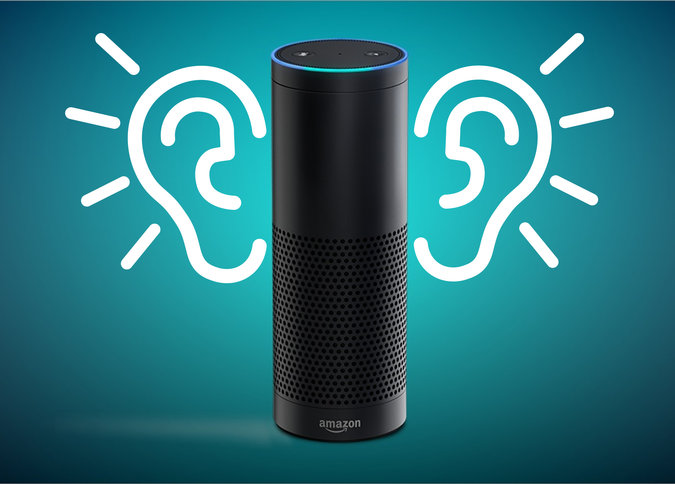
\includegraphics[width = 10cm]{ucho.jpg} 
\end{center}
\end{figure}

\vspace{9mm}

\begin{tabular}{rl}

Autoři: & Jiří Burant \\
\noalign{\vspace{1mm}}
		& Jakub Drápela \\
		\noalign{\vspace{1mm}}
		& Martin Klučka\\
		\noalign{\vspace{1mm}}
		& Petr Kovář \\
		\noalign{\vspace{1mm}}
		& Jakub Konrád\\
		\noalign{\vspace{1mm}}
		& Pavel Trutman\\
\noalign{\vspace{2mm}}
Studijní obor: & Kybernetika a robotika \\
\noalign{\vspace{2mm}}
Datum vypracování: & \today\\
\end{tabular}

\end{center}

\newpage
\pagestyle{plain}     % zapne obyčejné číslování
\setcounter{page}{1}
%% zahlaví a zápatí
\addtolength{\voffset}{-3cm}
\addtolength{\headheight}{2cm}

\pagestyle{fancy}
\lhead{
\includegraphics[scale=0.12]{cvut_text.jpg}  }
\chead{\textbf{Household Intelligent Assistant}}
%\rhead{\textit{\bfseries Burant,Drápela,Klučka,Kovář,Konrád,Trutman}}
\lfoot{}
\cfoot{\thepage}
\rfoot{}
\renewcommand{\headrulewidth}{0.4pt}

%jakékoliv změny povoleny, všude....
%prvotní nepřečtený návh - jdu běhat, pak se na to zase kouknu :)

\section*{Popis projektu, motivace}


Jako lidi si klademe různé otázky. Abychom mohli ve světě rozumě fungovat potřebujeme znát odpovědi na ně. Od té doby, co se začaly informace zaznamenávat lze odpovědi nalézt v záznamech. V nedávné historii lidé prahnoucí po informacích ve velkém kupovali knihy, noviny, jízdní řády, prostě média se žádaným obsahem. 

Doba pokročila. My jsme se posunuly do doby, kde jsou téměř všechny informace uložené v elektronické podobě. Je běžné k nim přistupovat pomocí moderních přístrojů. Téměř každý aktivní člověk vlastní alespoň jednu z věcí, jako je počítač, notebook, chytrý mobilní telefon, tablet, iPad a jiné. S využitím toho vybavení máme značně usnadněnou cestu k získání potřebné informace. Stačí mít u sebe správnou aplikaci, přístup na internet a například dopravní spojení nalezneme do minutky. Limituje nás ovšem schopnost manipulace, což při troše nešikovnosti dokáže člověka dost rozčílit.

My se snažíme jít o krok vpřed. Ruční manipulaci obejít a informace získávat pouze pomocí našeho vlastního hlasu, což ovšem obsahuje širokou škálu požadavků.  

\section*{Detailní specifikace}
V našem projektu se zaměříme na vytvoření dialogového systému pro použití v běžné domácnosti či kanceláři. Tedy systému, který dovede sám odpovídat na kladené otázky z limitované oblasti počasí, dopravy, obecných informací atd. Systém bude neustále čekat na aktivační slovo a potom bude schopen zodpovědět určitou škálu otázek. K realizaci projektu budeme využívat již existující aplikace. 
% napsat víc a víc

\section*{Popis navrženého řešení}
% možná detailněji
Při popisu návrhu řešení aplikace budeme postupovat tak, jak bude rekce na mluvené slovo postupně prostupovat mezi moduly, až nakonec vznikne finální řečená odpověď. Blokové schéma aplikace je zobrazeno na obrázku \ref{fig:diagram api}.

V prvotní situaci bude aplikace v režimu čekání na aktivační slovo. Na rozpoznání aktivačního slova bude vyhrazen jedem samostatný modul. Aktivační slovo by mělo být snadno oddělitelné od ostatních. Ukazuje se vhodné zvolit tříslabičné slovo s výraznými písmeny jako je např. x.

Po zaznění aktivačního slova uživatelem se aktivuje blok pro rozpoznání mluveného slova. Vhodnou robustní aplikací pro tento problém je třeba vybrat. Experimentovat budeme s \textit{wit.ai} a \textit{PocketSphinx}.

\begin{figure}[h!]
	\begin{center}
	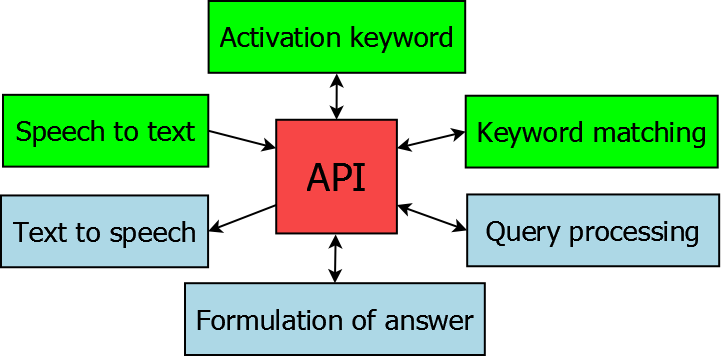
\includegraphics[width = 14cm]{Diagram_API.png}
	\caption{Blokový diagram navrženého řešení projektu Household Intelligent Assistant}
	\label{fig:diagram api}
	\end{center}
\end{figure}

Ze získaného textu je třeba vybrat klíčová slova, která definují otázku v různých formulacích. Klíčová již rozezná například již zmiňovaná aplikace \textit{PocketSphinx}.


Získaná klíčová slova jsou vstupní hodnotou do modulu, jenž získá potřebné informace z internetu. Úlohy budou rozdělené na jednotlivé subsystémy. Jeden subsystém bude například pouze na zpracování odpovědi na počasí. 

Odpověď kterou dostaneme je třeba přeformulovat do srozumitelné odpovědi podle předem zadaných vzorů. 

V poslední řadě využijeme aplikaci k převedení formulované odpovědi do strojově mluvené řeči. Prvotní aplikací pro tento může být jednoduchý "The Festival Speech Synthesis System".

% plus dopsat nějaké kecy kolem 


\section*{Plánování projektu(Ganttův diagram, úkoly, milníky)}

\section*{Analýza rizik a krizové plány}

\section*{Předběžné výsledky}

Zdroje:
http://static01.nyt.com/images/2015/06/25/business/GADGETWISE/GADGETWISE-master675.jpg
\end{document}
